\section{Introduction}
\subsection{History of Programmable Logic}


\begin{description}
\item [TTL(Transistor Transistor Logic) logic design] Implementng logic by using basic logic funtions available on separate chips/ ICs (ex: Texas Instruments 7400 device family) on a breadboard. Methodology: 
    \begin{itemize}
    \item Creating truth table.
    \item Cration Karnaugh map.
    \item Generate logical expression.
    \item Final logic implementation.
    \end{itemize}

\item [Programamble logic] 
    \begin{description}
    \item  [Programamble Array Logic(PAL)] Simplest implementation of programmable logic. Logic gates and registers fixed. 
    Programmable sum of products array and output control. Floating-gate transistors at array crossings set to never conduct after applying programming voltages.
    \\ Put image here

    \item [Programamble Logic Devices (PLD)] Arrange multiple PAL arrays in a single device. It is comprised of: i. Variable product term distribution ii. Programmable macrocells

    Programmable macrocells:
    Generated programmable output from sum of products. Provided feedback (using output pin as input)

    \end{description}

\item [Complex Programamble Logic Devices (CPLD)] Combine multiple PLDs(logic blocks) in a single device with programmable interconnect and I/O.

Put image here:

CPLD logic block or Logic Array Blocks(LAB):

Contain multiple macrocells (typically 4 to 20)
Local programmable interconnect like a PLD.




\item [Other architectures]

    \begin{description}
    \item [Programmable Interconnect Array(PI or PIA)] Similar to PAL programming technology. Global routing connects any signal to any destination in device. Programmed wih EPROM,EEPROM or flash technology.

    \item [I/O control blocks] Introduction in CPLDs. Seprated from logic by PI. I/O specific logic provides control, more features. Tri-state buffer control to enable input, outputs, or bidirectional on any I/O pin.

    \item [In-System Programming (ISP) with JTAG] Simple 4 or 5 wire serial interface. Shifts data through one or more devices on a board (JTAG chain). Used for device self test or ISP.
PLD Hardware generates EEPROM programming voltages controlled by JTAG interface.

    \end{description}


\end{description}

\subsection{What is an FPGA?}
FPGA stands for field-programmable gate array, and it's a special type of integrated circuit that implements an arbitrary digital design of one's own. FPGA is an integrated circuit consisting of an array of programmable logic blocks with programmable routing between the blocks, that allows the device to be configured to perform complex digital logic functions. In other words, the code determines the configuration of the digital circuitry inside the chip. 

FPGAs are the key technology enabling many of the great new product developments in the near future. Including autonomous vehicles, the Internet of Things, secure data centers and cloud computing, robotics, machine vision and learning, renewable energy, home automation, 8K video and video surveillance, facial recognition and bioinformatics, 5G cellular networks, and smart medical diagnostics.

So how is an FPGA customized? We can sum it all up in three steps. 
\begin{itemize}
	\item The system is designed as source code in a hardware description language like VHDL or Verilog. 
	\item The code is synthesized by a software tool essentially similar to a compiler. FPGA synthesis is the process of taking the source code and producing an output file that describes the internal connections that the FPGA needs in order to become one's design. 
	\item The output file is downloaded into the FPGA, which has a special memory for this binary data.
\end{itemize}

\subsection{FPGAs are not microcontrollers}
FPGAs may sound similar to microcontrollers, but it's very important to understand the difference. First, FPGAs are flexible in that they customize their internal connections. On the other hand, microcontrollers can't behave as anything other than microcontrollers. They are application-specific integrated circuits, or ASIC. Next, remember that an FPGA may implement a CPU, so technically, an FPGA can achieve more than a microcontroller. Another key difference is that FPGAs do not execute code, microcontrollers do. And finally, embedded systems were originally based in microcontrollers or microprocessors, and over the years they have evolved to include FPGAs as well.\\\\
Suggested Readings:
\begin{itemize}
	\item FPGAs for Dummies, Altera Version, available here:  http://design.altera.com/New2FPGAeBook, Chapters 1, 2, and 5 (27 pages).
	\item Rapid Prototyping of Digital Systems: SOPC Edition, by Hamblen, Hall and Furman; ISBN 9780387726700, Chapter 3 (14 pages)
	\item Design Recipes for FPGAs Using Verilog and VHDL, 2nd Edition, by Peter Wilson, Chapter 2 (7 pages)
\end{itemize}


\subsection{Programmable Logic Devices (PLD)}
FPGAs are a subset programmable logic devices. 
\begin{figure}[H]
	\begin{center}
		\includegraphics[width=5in]{images/PLD.png}
		\caption{PLD Classification}
		\label{PLD}
	\end{center}
\end{figure}


CPLD (Complex Programmable Logic Devices):\\
CPLDs have several useful characteristics, including easy generation of wide input functions, and easy to calculate timing that is very predictable. It's said to be deterministic. They are still a good choice for glue logic applications today. However, for designs that required a lot of registers, data transfers, bus interfaces. These logic intensive flip-flop scarce devices did not scale well, leading to the development of another PLD architecture,the FPGA.


CPLD re-introduced reprogrammability to programmable logic devices, an important new feature. CPLDs also reinforced hierarchical design methods. The architecture of the CPLD allowed for easy design of wide input combinational logic functions like address decoders and state machines with deterministic timing. However, the CPLD architecture did not scale effectively for designs that required many flip flips. This has become the province of the FPGA.

FPGA vs PLD vs ASIC:

\subsubsection{Programmable Logic Devices}
Highly configurable
Fast Design Time
Can't support complex logic
SPLD: Simple PLD
CPLD: Complex PLD
\subsubsection{Application Specific Integrated Circuits}
No reconfiguration
Application Specific
Area and power optimized
Time consuming design
Highly expensive
Supports complex logic
\subsubsection{FPGAs}
FPGAs sit in tbetween these two extemities.
Reconfigurable
Inexpensive
Easy to program
Reprogrammable chip
Time to market is less (~ a month as opposed to ASIC which needs around 6-8 months)
Can be used as a "Glue logic" in order to connect large ICs.
Reduces system complexity
Density of FPGA continue to grow (gates/area)
FPGA prototyping for ASIC verification

\begin{table}[H]
\begin{center}
\begin{tabular}{@{}llll@{}}
\toprule
\textbf{Performance} & \textbf{Non recurring cost} & \textbf{Unit Cost} & \textbf{Time to Market} \\ \midrule
ASIC                 & ASIC                        & FPGA               & ASIC                    \\
FPGA                 & FPGA                        & Microprocessor     & FPGA                    \\
Microprocessor       & Microprocessor              & ASIC               & Microprocessor          \\ \bottomrule
\end{tabular}

\end{center}
\end{table}

\section{FPGA Architecture}

\subsection{Intel FPGA Architechture}

FPGA Logic Array Blocks (LABs) are made up of Logic Elements (LEs) or Adaptive Logic Modules (ALMs). Each of these logic blocks consists of Look Up Tables(LUTs), and registers.

\subsubsection{Look Up Tables(LUTs)}
Creating sum of products function out of combinatorial logic in an FPGA. FPGA uses four or more input LUTs to create complicated functions. A LUT is made up of a series of cascaded multiplexers where the LUT inputs are used as the select lines. The inputs to the multiplexers are programmed as hugh ir low logic levels. The logic is called a Look Up Table.

\subsubsection{Programmable Register}
This is the synchronous part of an Logic Elements. It is driven by a global device clock. Aynchronous control signals of the registers(ex. clear, reset) can be generated by other logic or come from an I/O pin. The output of the register can drive out of the LE to the device's routing channels, or be fed back into the LUT. Register could be bypassed for a combinatorial logic. LUT could also be bypassed and only register could be used for memory. This flexibility in the output stage of the LE makes it extremely efficient.

\subsubsection{Carry and Register chains}
Chains carry bits between LEs. Register outputs can chain to other LE registers in LAB toform LUT independent shift registers. 

\textbf{Register packing}\\
FPGA LEs can be configured to perform a function called Register packing. Two seperate functions can be output from a single LE, one from the carry and chain logic and the other from the output register. This helps in saving device resources.

\subsubsection{Adaptive Logic Module (ALM)}
Replacement for the LEs from traditional FPGAs due to lack of cascading and feedback which is necessary to generate functions with more inputs than are available. It improves performance and resource utilization. ALMS comprise of 2 to 4 output registers to provide even more options for logic chaining, register packing, and generating multiple functions within a single logic block. ALMs also have dedicated built-in hardware adder blocks. The main differentiator between LEs and LUTs is a LUT. The LUT in an ALM is an Adaptive LUT or ALUT. ALUT can be split and configured into different sized LUTs to accommodate two separate functions.

FPGA Routing:\\
In an FPGA, the LABs are all arranged into a large array. Programmable routing is placed in the spaces between LABs, similar to the streets in a city. 

\subsection{Intel Products}
Intel delivers a broad portfolio of custom logic solutions such as FPGAs, SoCs, structured ASICs, and CPLDs together with software tools, intellectual property (IP), embedded processors, customer support, and technical training.
\subsubsection{Intel FPGAs}
\begin{description}
    \item[Intel Agilex FPGAs] This FPGA family integrate an 10nm FPGA. Intel Agilex SoC FPGAs integrate the quad-core Arm Cortex-A53 processor. Applications: wide range of compute and bandwidth intensive applications. 
    \item[INTEL AGILEX F-SERIES FPGAs AND SoCs] This FPGA and SoC FPGA family bring together transceiver support, digital signal processing (DSP) capabilities along with an option to integrate the quad-core Arm Cortex-A53 processor. Applications: wide range of data center, networking, and edge applications.
    \item[INTEL AGILEX I-SERIES SoC FPGAs] This FPGA family is optimized for high-performance processor interface and bandwidth-intensive  applications.  
    \item[INTEL AGILEX M-SERIES SoC FPGAs] This SoC FPGA family is optimized for compute and memory intensive applications. 
    \item[Intel Stratix Series] This FPGA and SoC family enables you to deliver high-performance, state-of-the-art products to market faster with lower risk and higher productivity. 
    \item[Intel Arria Series] This device family delivers performance and power efficiency in the midrange. The Intel Arria 10 FPGAs and SoCs are ideal for the end market applications such as Wireless, Cloud Service and Storage, Broadcast.
    \item[Intel Cyclone Series] The Intel Cyclone FPGA series is built to meet your low-power, cost-sensitive design needs, enabling you to get to market faster.
    \item[Intel MAX Series] This non-volatile FPGA family is optimized for a wide range of high-volume, cost-sensitive applications, such as Automotive, Industrial, Communications.
\end{description}
\subsubsection{Intel eASIC Devices}
Intel eASIC devices are structured ASICs, an intermediary technology between FPGAs and standard-cell ASICs, that provide lower unit cost and lower power compared to FPGAs. These devices provide faster time to market and lower non-recurring engineering (NRE) cost compared to standard-cell ASICs.
Different eASIC amilies are: Intel eASIC N5X Devices (Comes with Arm Cortex-A53 hard processor system), Intel eASIC N3XS Devices, Intel eASIC N3X and N2XT Devices.
\subsection{Plain FPGA / Inside an FPGA: Logic blocks}

There are many basic elements inside FPGAs that make it possible to provide the arbitrary functionality we want. Here are the most basic of these elements. First we have logic blocks, which contain the logic elements that finally implement one's design. These include digital devices like lookup tables, flip-flops and multiplexers. Next we have the inter-connect block, which is an enormous network of switches that route the logic elements to connect them as one's design requires. I/O blocks contain the circuitry for input and output things in the integrated circuit. Most FPGAs contain memory blocks to implement large arrays, and also a clock management block to implement sequential systems. 

\subsubsection{Logic blocks} 
These are also known as configurable logic blocks or CLB's. Each logic block contains a number of logic cells which are smaller groups of basic logic elements. Although the letter G in FPGA stands for Gate, logic cells don't usually contain gates. Real logic cells may have these elements, like types of flip-flops, D multiplexers, larger lookup tables, small register arrays, and so on.\\

\par \textbf{Lookup Tables} FPGAs use LUTs of various sizes to implement logic. There's a tradeoff between the size of the LUT and the amount of routing required. Larger LUTs can create more logic, which will require less routing. Smaller LUTs will require more routing, but offer better logic efficiency. LUTs can be used to create a variety of combinatorial logic functions.

\textbf{Flip-flops / Register} A flip-flop is a circuit that has two stable states and can be used to store state information. A flip-flop is a device which stores a single bit of data; one of its two states represents a "one" and the other represents a "zero". Such data storage can be used for storage of state, and such a circuit is described as sequential logic in electronics. A flip-flop usually comprises of a clock(CLK), input(D) and an output(Q) signal.

A clock signal oscillates between a high and a low state (an analog square wave) and is used like a metronome to coordinate actions of digital circuits. FPGAs usually runs on a clock with a MHz frequency. This clock runs multiple Flip-flops inside an FPGA. These Flip-flops operate on the clock edges (usually the rising edge).

Types: D FF, JK FF, T FF.

\begin{itemize}
	\item D Flip-flop: Aligns input data to the clock edges.
	\begin{figure}[H]
        \begin{center}
            \includegraphics[width=4in]{images/D-FF.png}
            \caption{D Flip Flop}
            \label{DFF}
        \end{center}
    \end{figure}

    \begin{figure}[H]
        \begin{center}
            \includegraphics[width=4in]{images/D-FF-Timing.png}
            \caption{Timing diagram of D Flip flop}
            \label{DFFTime}
        \end{center}
    \end{figure}

	\item JK Flip-flop
	\item T Flip-flop
\end{itemize}

\subsubsection{Interconnects}
This is the part of the FPGA that has all the custom connections between logic cells across logic blocks. The interconnects are typically implemented by switch boxes which contain a number of simple semiconductor switches. Each of these switches is either open or closed depending on a logic state in it's input. These open or closed states come from a special memory in the FPGA.

\begin{figure}[H]
	\begin{center}
		\includegraphics[width=5in]{images/ICSwitch.png}
		\caption{Switch Box}
		\label{SwitchBox}
	\end{center}
\end{figure}

This is how a switch box may be implemented in \figref{SwitchBox}. At the left we have six different wires that may be connected between each other in any way. This is possible because there are switch boxes at the intersections. Now look This is how a switch box may be implemented. ing closer at the switch box, it may contain as many as six switches to route any signal in any direction needed. If one look carefully, one'll see that a single switch box is capable of routing two different signals. For example, one that goes horizontally and one that goes vertically through the switch box. 

\begin{figure}[H]
	\begin{center}
		\includegraphics[width=5in]{images/IC.png}
		\caption{Interconnect}
		\label{Interconnect}
	\end{center}
\end{figure}

Interconnect seems simple enough and they are very simple indeed as shown in \figref{Interconnect}. But the real power in an FPGA comes from the enormous number of interconnects available. An FPGA has so many interconnects that it's humanly impossible to create a design by hand. This huge network architecture is sometimes called an interconnect fabric and it requires software to keep track of all of the routing that needs to be done.

Aside from logic block and interconnects there are many more important elements in an FPGA for eg. I/O blocks, clock management blocks, memory blocks, and hard I/P cores.

\subsubsection{I/O blocks}
Input/Output blocks are always included in FPGAs because integrated circuits work with very low powers, voltages and currents internally. However, the outside world usually works with higher powers. That's why I/O blocks contain line drivers to provide power to the outputs, and line receivers to condition the incoming signals to the lower internal power levels. I/O blocks also contain protection devices to avoid damage from external conditions, such as electrostatic discharges. Output pins can sometimes customize other perameters like strength or speed of the outgoing signal.

\subsubsection{Clock management blocks}
These are usually provided in FPGAs because virtually all useful systems are sequential, and thus require a clock signal. External oscillators are almost always required. This is not the usual case with microcontrollers which may contain an internal, good enough oscillator. There are several features in a clock manager, but most are related with changing the incoming frequency to some other frequency. So one can reduce it by some factor with a rescaler, or one can boost it up with a control system called a phase-locked loop or PLL. 

\subsubsection{Memory blocks}
Memory blocks are almost always included because most applications require RAM and ROM. Because the digital design that will be written to an FPGA is not known in advance, these memories have to support segmentation to meet the programmers needs. These are general purpose memories with at risk inputs and data lines. These memories are available from the source code as memory blocks defined in the hardware description language. Finally, the interconnects take care of the segmentation. 

\subsubsection{Hard IP Cores}
A very special part of the FPGA world are IP cores. Intellectual property cores are functional blocks available for use. This can be provided in libraries for one to use in the code, or they can be hardware blocks like the ones available in most microcontrollers. Hard IP cores are accessible from one's code as if they were instances of logic designs. Having these available in hardware helps keeping one's custom designs smaller, and speeds up the development process. Some examples of Hard IP cores are HDMI controllers, serial ports, CPUs, digital signal processors, and USB controllers.

\subsection{System on Chip / SoC}
A System on a Chip or a System on Chip (SOC) is an integrated circuit that integrates all components of a computer into an electronic system into a single chip. It may contain digital, analog, mixed-signal and other radio frequency functions on a single chip substrate. SOCs are very common in the mobile electronics market because of their low power consumption. Another typical application is in the area of embedded systems. Another definition for a System on a Chip or System on Chip is an integrated circuit that integrates more than one component into a single chip along with a CPU. Typical component types are GPUs, communication interfaces, analog functions, and radios. If it includes programmable logic then it is a programmable SoC, or an SoC FPGA. The higher integration of an SoC provides lower cost, smaller size, and lower power than alternatives. 

Heavylifting is done on the FPGA and rest with less computation time (non real time) is done on the processor part. Zynq architecture fusion of a processor(PS) and an FPGA(PL). They communicate with AXI protocols. Zynq is mainly used for acceleration. Processor with FPGA work together to get higher operation speeds. Application include: Image processing, DSP etc. 

\subsubsection{Software Profiling} What to put in FPGA and what to put in the processor.

\pagebreak
\section{Timing Analysis}

\subsection{Introduction}
Timing analysis is the methodical analysis of a digital circuit to determine if the timing constraints imposed by components or interfaces are met. Typically, this means that you are trying to meet all set-up, hold, and pulse-width times requirement.\\ During designing there is a trade-offs between speed, area, power, and runtime according to the constraints set by the designer. However, a chip must meet the timing constraints to operate at the intended clock rate, so timing is the most important design constraint.

\subsection{Reasons for performing Timing Analysis}
\begin{itemize}
    \item To verify whether the design meets all the timing requirements.
    \item To verify that the design for all combinations of components over the entire specified operating environment at every time instance. 
    \item Timing analysis can also help with component selection.
\end{itemize}

\subsection{Types of Timing Analysis}

There are 2 type of Timing Analysis:
\begin{itemize}
    \item \textbf{Static Timing Analysis:} Checks static delay requirements of the circuit without any input or output vectors.
    \item \textbf{Dynamic Timing Analysis:} verifies functionality of the design by applying input vectors and checking for correct output vectors.
\end{itemize}

The basis of all timing analysis are the "Clock" and "Sequential component" (Flip-flop, Latches) of the design. Following are a few directives related to clock and Flip-Flop for Timing analysis.
\subsubsection{Clock directives}
\begin{itemize}
    \item Clock must be well understood parametrically and glitch-free.
    \item Timing analysis must ensure that any clock that is generated by the digital logic is clean, of bounded period \& duty cycle, and of a known phase relationship to other clock signals of interest.
    \item The clock must, for both high and low phases, meet the minimum pulse width requirements.
    \item Certain circuits, may require monitoring maximum jitter. Jitter might become a critical parameter, with higher clock speeds.
    \item When "passing" data from one clock edge to the other, one has to ensure that the worst-case duty cycle is used for the calculation. Remember: A frequent source of error is the designer assuming that every clock will have a 50\% duty cycle.
\end{itemize}
\clearpage
\subsubsection{Flip-Flop directives}
\begin{itemize}
    \item Make sure that all the parameters of Flip-Flops always met. The only exception is when synchronizers are used to synchronize asynchronous signals.
    \item For asynchronous presets and clears, Recovery and Removal constraints must be met.
    \item All setup and hold times are met for the earliest/latest arrival times for the clock.
    \item Setup times are generally calculated by designers and suitable margins can be demonstrated under test. Hold times, however, are frequently not calculated by designers.
    \item When passing data from one clock domain to another, ensure that there is either known phase relationships which will guarantee meeting setup and hold times or that the circuits are properly synchronized.    
\end{itemize}

\section{Static Timing Analysis (STA)}
\subsubsection{Definition}
Static timing analysis (STA) is a method of validating the timing performance of a design by checking all possible paths for timing violations under worst-case conditions. STA is more thorough because it checks the worst-case timing for all possible logic conditions, not just those sensitized by a particular set of test vectors. However, STA can only check the timing, not the functionality, of a circuit design unlike functional simulation.

\subsubsection{Description} 
In static timing analysis, the word static alludes to the fact that this timing analysis is carried out in an input-independent manner. There are huge numbers of logic paths inside a chip of complex design. The advantage of STA is that it performs timing analysis on all possible paths (whether they are real or potential false paths). However, it is worth noting that STA is not suitable for all design styles. It has proven efficient only for fully synchronous designs. Since the majority of chip design is synchronous, it has become a mainstay of chip design over the last few decades.\\
Static timing analysis involves following steps: 
\begin{enumerate}
    \item Breaks a design down into timing paths.
    \item Calculates the signal propagation delay along each path.
    \item Checks for violations of timing constraints inside the design and at the input/output interface.
\end{enumerate}

\subsection{Timing Paths}
When performing timing analysis, STA first breaks down the design into timing paths. Each timing path consists of the following elements:
\begin{enumerate}
    \item \textbf{Startpoint} The start of a timing path where data is launched by a clock edge or where the data must be available at a specific time. Every startpoint must be either an input port or a register clock pin.
    \item \textbf{Combinatorial logic network} Elements that have no memory or internal state. Combinatorial logic can contain AND, OR, XOR, and inverter elements, but cannot contain Flip-Flops, latches, registers, or RAM.
    \item \textbf{Endpoint} The end of a timing path where data is captured by a clock edge or where the data must be available at a specific time. Every endpoint must be either a register data input pin or an output port.
\end{enumerate}

\begin{figure}[H]
\begin{center}
\includegraphics[width=4.5in]{images/STAPaths.jpg}
\caption{Timing paths in a simple design example}
\label{STAPaths}
\end{center}
\end{figure}

A combinatorial logic cloud might contain multiple paths, as shown in the \figref{STAMultipath}. STA uses the longest path to calculate a maximum delay and the shortest path to calculate a minimum delay.

\begin{figure}[H]
\begin{center}
\includegraphics[width=4in]{images/STAMultipath.jpg}
\caption{Multiple timing paths in a combinatorial logic}
\label{STAMultipath}
\end{center}
\end{figure}

The STA tool analyzes all the paths from each and every startpoint to each and every endpoint and compares it against the constraint that (should) exist for that path. All paths should be constrained, most paths are constrained by the definition of the period of the clock, and the timing characteristics of the primary inputs and outputs of the circuit.
\clearpage
\subsection{Types of Timing Paths}
There are 4 types of Timing Paths:
\begin{enumerate}
    \item Data Path
    \item Clock Path
    \item Clock Gating Path
    \item Asynchronous Path 
\end{enumerate}

\begin{figure}[H]
\begin{center}
\includegraphics[width=4.5in]{images/STAPathTypes.jpg}
\caption{Types of timing paths in a combinatorial logic}
\label{STAPathTypes}
\end{center}
\end{figure}

Each of the Timing Paths, is explained with the help of \figref{STAPathTypes} in sections below.

\subsubsection{Data path}
Data path is a path from a clock input port or Clock pin, through the Flip-Flop/latch/memory (sequential cell), to the Data input pin of the sequential element.

\begin{itemize}
    \item Start Point: Input port of the design (for data from some external source) or,\\ Clock pin of the Flip-Flop/latch/memory (sequential cell).
    \item End Point: Data input pin of the Flip-Flop/latch/memory (sequential cell) or, \\ Output port of the design (for the data captured by some external sink).
\end{itemize}

\paragraph{Types of Data Paths}
With the combination of 2 types of Starting Points and 2 types of End Points, there are 4 types of Timing Paths, which are mentioned below:
\begin{enumerate}
    \item Input pin/port to Register(Flip-Flop). 
    \item Input pin/port to Output pin/port.
    \item Register (Flip-Flop) to Register (Flip-Flop)
    \item Register (Flip-Flop) to Output pin/port
\end{enumerate}

\begin{figure}[H]
\begin{center}
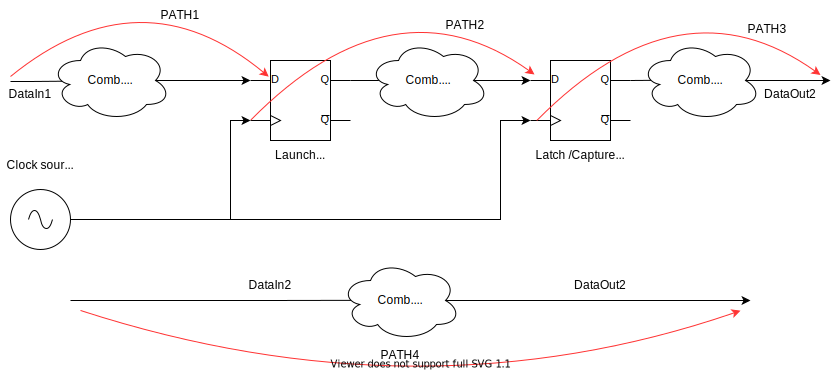
\includegraphics[width=\textwidth]{images/STADataPath.png}
\caption{Types of Data Paths in a combinatorial logic}
\label{STADataPath}
\end{center}
\end{figure}

\begin{itemize}
    \item PATH1- starts at an input port and ends at the data input of a sequential element. (Input port to Register)
    \item PATH2- starts at the clock pin of a sequential element and ends at the data input of a sequential element. (Register to Register)
    \item PATH3- starts at the clock pin of a sequential element and ends at an output port.(Register to Output port).
    \item PATH4- starts at an input port and ends at an output port. (Input port to Output port)
\end{itemize}

\subsubsection{Clock Path}
As per \figref{STAPathTypes}, Clock path is a path from a clock input port or cell pin, through one or more buffers or inverters, to the clock pin of a sequential element for data setup and hold checks. In between the Start point and the end point there may be lots of Buffers/Inverters/clock divider.

\begin{itemize}
    \item Start Point: Clock input port
    \item End Point: Clock pin of the Flip-Flop/latch/memory (sequential cell)
\end{itemize}

\subsubsection{Clock Gating Path}
As per \figref{STAPathTypes}, Clock path may be passed trough a gated element to achieve additional advantages. this type of clock path is called as gated clock path. Clock gating path is a path from an input port to a clock-gating element for clock gating setup and hold checks.

\begin{itemize}
    \item Start Point: Input port of the design
    \item End Point: Input port of clock-gating element.
\end{itemize}

\subsubsection{Asynchronous path}
As per \figref{STAPathTypes}, asynchronous path is a path from an input port to an asynchronous set or clear pin of a sequential element; for recovery and removal checks.

\begin{itemize}
    \item Start Point: Input port of the design
    \item End Point: Set/Reset/Clear pin of the Flip-Flop/latch/memory (sequential cell)
\end{itemize}

As you know that the functionality of set/reset pin is independent from the clock edge. Its level triggered pins and can start functioning at any instance of time. In other words, this path is not synchronous with the rest of the circuit and hence is called as Asynchronous path.

\subsection{Other types of Paths}
There are few more types of path which are used during timing analysis. Those are a subset of above mentioned paths with some specific characteristics. Other types of Paths include:
\begin{itemize}
    \item Critical path
    \item False Path
    \item Multi-cycle path
    \item Single Cycle path
    \item Launch Path
    \item Capture Path
    \item Longest Path ( Also know as Worst Path, Late Path, Max Path, Maximum Delay Path)
    \item Shortest Path ( Also Know as Best Path, Early Path, Min Path, Minimum Delay Path)
\end{itemize}

\iffalse
\subsubsection{Critical Path}
In short, I can say that the path which creates Longest delay is the critical path.
Critical paths are timing-sensitive functional paths. because of the timing of these paths is critical, no additional gates are allowed to be added to the path, to prevent increasing the delay of the critical path.
Timing critical path are those path that do not meet your timing. What normally happens is that after synthesis the tool will give you a number of path which have a negative slag. The first thing you would do is to make sure those path are not false or multicycle since it that case you can just ignore them.
Taking a typical example (in a very simpler way), the STA tool will add the delay contributed from all the logic connecting the Q output of one flop to the D input of the next (including the CLK-&gt;Q of the first flop), and then compare it against the defined clock period of the CLK pins (assuming both flops are on the same clock, and taking into account the setup time of the second flop and the clock skew). This should be strictly less than the clock period defined for that clock. If the delay is less than the clock period, then the "path meets timing". If it is greater, than the "path fails timing". The "critical path" is the path out of all the possible paths that either exceeds its constraint by the largest amount, or, if all paths pass, then the one that comes closest to failing.


False Path:
Physically exist in the design but those are logically/functionally incorrect path. Means no data is transferred from Start Point to End Point. There may be several reasons of such path present in the design.
Some time we have to explicitly define/create few false path with in the design. E.g for setting a relationship between 2 Asynchronous Clocks. 
The goal in static timing analysis is to do timing analysis on all true timing paths, these paths are excluded from timing analysis. 
Since false path are not exercised during normal circuit operation, they typically don't meet timing specification,considering false path during timing closure can result into timing violations and the procedure to fix would introduce unnecessary complexities in the design.
<li style="border-bottom: medium none; border-left: medium none; border-right: medium none; border-top: medium none;">There may be few paths in your design which are not critical for timing or masking other paths which are important for timing optimization, or never occur with in normal situation. In such case , to increase the run time and improving the timing result , sometime we have to declare such path as a False path , so that Timing analysis tool ignore these paths and so the proper analysis with respect to other paths. Or During optimization don't concentrate over such paths. One example of this. e.g A path between two multiplexed blocks that are never enabled at the same time. You can see the following picture for this.

<table align="center" cellpadding="0" cellspacing="0" class="tr-caption-container" style="margin-left: auto; margin-right: auto; text-align: center;"><tbody>
<tr><td style="text-align: center;"><a href="https://lh4.googleusercontent.com/-nb0f6wv3c60/TXCmhNOHMaI/AAAAAAAAACs/il_jOYJEH8U/s1600/false+path.bmp" imageanchor="1" style="margin-left: auto; margin-right: auto;"><img border="0" height="191" l6="true" src="https://lh4.googleusercontent.com/-nb0f6wv3c60/TXCmhNOHMaI/AAAAAAAAACs/il_jOYJEH8U/s400/false+path.bmp" width="400" /></a></td></tr>
<tr><td class="tr-caption" style="text-align: center;">False Path</td></tr>
</tbody></table><div style="border-bottom: medium none; border-left: medium none; border-right: medium none; border-top: medium none; text-align: left;">
Here you can see that False path 1 and False Path 2 can not occur at the same time but during optimization it can effect the timing of another path. So in such scenario, we have to define one of the path as false path.</div>
Same thing I can explain in another way (Note- Took snapshot from one of the forum). As we know that, not all paths that exist in a circuit are "real" timing paths. For example, let us assume that one of the primary inputs to the chip is a configuration input; on the board it must be tied either to VCC or to GND. Since this pin can never change, there are never any timing events on that signal. As a result, all STA paths that start at this particular startpoint are false. The STA tool (and the synthesis tool) cannot know that this pin is going to be tied off, so it needs to be told that these STA paths are false, which the designer can do by telling the tool using a "false_path" directive. When told that the paths are false, the STA tool will not analyze it (and hence will not compare it to a constraint, so this path can not fail), nor will a synthesis tool do any optimizations on that particular path to make it faster; synthesis tools try and improve paths until they "meet timing" - since the path is false, the synthesis tool has no work to do on this path.
Thus, a path should be declared false if the designer KNOWS that the path in question is not a real timing path, even though it looks like one to the STA tool. One must be very careful with declaring a path false. If you declare a path false, and there is ANY situation where it is actually a real path, then you have created the potential for a circuit to fail, and for the most part, you will not catch the error until the chip is on a board, and (not) working. Typically, false paths exists

from configuration inputs like the one described above
from "test" inputs; inputs that are only used in the testing of the chip,and are tied off in normal mode (however, there may still be some static timing constraints for the test mode of the chip)
from asynchronous inputs to the chip (and you must have some form of synchronizing circuit on this input) (this is not an exhaustive list, but covers the majority of legitimate false paths).
So we can say that false paths should NOT be derived from running the STA tool (or synthesis tool); they should be known by the designer as part of the definition of the circuit, and constrained accordingly at the time of initial synthesis.

MultiCycle Path:A multicycle path is a timing path that is designed to take more than one clock cycle for the data to propagate from the startpoint to the endpoint.

A multi-cycle path is a path that is allowed multiple clock cycles for propagation. Again, it is a path that starts at a timing startpoint and ends at a timing endpoint. However, for a multi-cycle path, the normal constraint on this path is overridden to allow for the propagation to take multiple clocks.
In the simplest example, the startpoint and endpoint are flops clocked by the same clock. The normal constraint is therefore applied by the definition of the clock; the sum of all delays from the CLK arrival at the first flop to the arrival at the D of the second clock should take no more than 1 clock period minus the setup time of the second flop and adjusted for clock skew.
By defining the path as a multicycle path you can tell the synthesis or STA tool that the path has N clock cycles to propagate; so the timing check becomes "the propagation must be less than N x clock_period, minus the setup time and clock skew". N can be any number greater than 1.

Few examples are
When you are doing clock crossing from two closely related clocks; ie. from a 30MHz clock to a 60MHz clock, 
Assuming the two clocks are from the same clock source (i.e. one is the divided clock of the other), and the two clocks are in phase. 
The normal constraint in this case is from the rising edge of the 30MHz clock to the nearest edge of the 60MHz clock, which is 16ns later. However, if you have a signal in the 60MHz domain that indicates the phase of the 30MHz clock, you can design a circuit that allows for the full 33ns for the clock crossing, then the path from flop30 -&gt; to flop60 is a MCP (again with N=2). 
The generation of the signal 30MHZ_is_low is not trivial, since it must come from a flop which is clocked by the 60MHz clock, but show the phase of the 30MHz clock.
Another place would be when you have different parts of the design that run at different, but related frequencies. Again, consider a circuit that has some stuff running at 60MHz and some running on a divided clock at 30MHz. 
Instead of actually defining 2 clocks, you can use only the faster clock, and have a clock enable that prevents the clocks in the slower domain from updating every other clock, 
Then all the paths from the "30MHz" flops to the "30MHz" flops can be MCP. 
This is often done since it is usually a good idea to keep the number of different clock domains to a minimum.

\fi

\subsection{Setup and Hold Time}
Say, an Input "DIN" and an external clock "CLK" are buffered and passed through a combinational logic to reach a synchronous input and a clock input of a D Flip-Flop (say positive edge triggered). To capture the data correctly at D Flip-Flop, data should be present at the time of positive edge of clock signal at the Clk pin.

\begin{figure}[H]
\begin{center}
\includegraphics[width=4.5in]{images/STASetupHold.jpg}
\caption{Setup and Hold Time of the system}
\label{STASetupHold}
\end{center}
\end{figure}

Where,
\begin{itemize}
    \item \(T_{pdDIN}\): Propagation delay of DIN
    \item \(T_{pdClk}\): Propagation delay of CLK
    \item \(T_{s(in)}\): Setup time of the system
    \item \(T_{h(in)}\): Hold time of the system
    \item \(T_{s}\): Setup time of the D Flip-Flop
    \item \(T_{h)}\): Hold time of the D Flip-Flop
    \item DIN: System input
    \item CLK: System clock
\end{itemize}

In an ideal case, the setup and hold time would be zero. But still, 2 cases would arise.
\begin{itemize}
    \item \(T_{pdDIN} > T_{pdClk}\): For a successful capture, the data should be stable for \(T_{pdDIN} - T_{pdClk} = T_{S(in)}\) time at DIN pin before the positive clock edge at CLK pin. This Time "\(T_{s(in)}\)" is know as Setup time of the System.
    \item  \(T_{pdDIN} < T_{pdClk}\): For a successful capture, the data should remain stable for "\(T_{h(in)}\)" time at DIN pin after the positive clock edge at CLK pin. This time "\(T_{h(in)}\)" is know as Hold Time of the System.
\end{itemize}

From the above conditions, both the conditions are mutually exclusive. But we have to consider few more things in this.

\begin{itemize}
    \item Worst case and best case (Max delay and min delay): Considering the environmental \& Operating(PVT) conditions, analysis is performed for the worst case (max delay) and best case (min delay).
    \item Shortest Path or Longest path (Min Delay and Max delay): If a combinational logic has multiple paths, then the analysis is performed for the shortest path (min delay) \& longest path (max delay).
\end{itemize}

In other words,
\begin{itemize}
    \item \(T_{pdDIN(max)} > T_{pdClk(min)}\): \[Setup Time = T_{pdDIN(max)} - T_{pdClk(min)} \]
    \item  \(T_{pdDIN(min)} < T_{pdClk(max)}\): \[Hold Time = T_{pdClk(max)} - T_{pdDIN(min)} \]
\end{itemize}

When a hold check is performed we have to consider two things:
\begin{itemize}
    \item Minimum delay along the data path
    \item Maximum delay along the clock path 
\end{itemize}

When a setup check is performed we have to consider two things:
\begin{itemize}
    \item Maximum delay along the data path
    \item Minimum delay along the clock path 
\end{itemize}

\subsubsection{Definition}

\textbf{Setup time} is the minimum amount of time the data signal should be held steady before the clock event so that the data are reliably sampled by the clock. In other words, Setup time is the minimum amount of time required for the input of a Flip-Flop to be stable before the clock edge comes along.\\ 

\textbf{Hold time} is the minimum amount of time the data signal should be held steady after the clock event so that the data are reliably sampled. In other words, Hold time is the minimum amount of time required for the input of a Flip-Flop to be stable after the clock edge comes along.\\  

\begin{figure}[H]
\begin{center}
\includegraphics[width=4.5in]{images/STASetupHold2.jpg}
\caption{Setup and Hold Time Definitions}
\label{STASetupHold2}
\end{center}
\end{figure}

As the D Flip-Flop can be constructed with various implementations like, JK Flip-Flop, master slave Flip-Flop, Using 2 D type latches etc. Since, the internal circuitry is different for each type of Flip-Flop, the Setup and Hold time is different for every Flip-Flop.

\subsection{Setup and Hold Violation}
If the data is not stable before the Setup time calculated from active edge of the clock, there is a Setup violation at that Flip-Flop.\\ 
If the data is not stable after Hold time calculated from active edge of the clock, there is a hold violation at that Flip-Flop.

\begin{figure}[H]
\begin{center}
\includegraphics[width=4.5in]{images/STASetupHoldViolation.jpg}
\caption{Setup and Hold Time Violation}
\label{STASetupHoldViolation}
\end{center}
\end{figure}

\figref{TimingFF} is used to explain the Setup and Hold time Violation. The register transfer level is implemented on the hardware with VLSI technologies. The actual implemented hardware looks exactly like this instance of RTL from \figref{TimingFF}. This representation is the most commonly occurring structure inside any digital design hardware implementations. Two registers working on a single clock launching and capturing data with some form of combinatorial logic sitting between the two.

\begin{figure}[H]
\begin{center}
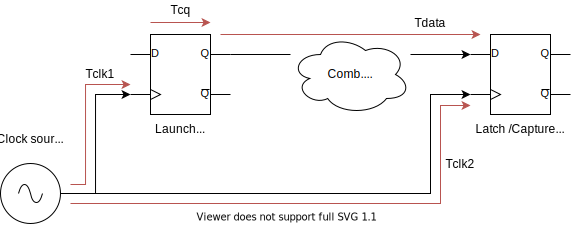
\includegraphics[width=\textwidth]{images/TimingFF.png}
\caption{Basic concepts of Timing Analysis}
\label{TimingFF}
\end{center}
\end{figure}

\begin{figure}[H]
\begin{center}
\includegraphics[width=\textwidth]{images/TimingDiaFF.png}
\caption{Timing Diagram}
\label{TimingDiaFF}
\end{center}
\end{figure}
    

\iffalse
Timing Diagram made from Wavedrom: https://wavedrom.com/
Source Code for timing diagram generation:
{signal: [
  {name: 'Source clk', wave: 'lh...l...h...l..'},
  {name: "TCLK1",   wave: "050......50....."},
  {name: 'FF1.clk', wave: 'l.h...l...h...l.'},
  {name: "Tcq",   wave: "l.50......50...."},
  {name: 'FF1.Q', wave: 'x..2...x...2...x', data: 'ValidData ValidData'},
  {name: "Tdata1",   wave: "l..50......5.0.."},
  {name: "Arrival time",   wave: "l5..0....5...0..", data: 'ArrivalTime1 ArrivalTime2'},
  {name: 'Source clk', wave: 'lh...l...h...l..'},  
  {name: "TCLK2",   wave: "07.0.....7.0...."},
  {name: 'FF2.clk', wave: 'l..h...l...h...l'},  
  {name: "Setup Hold",   wave: "0.340.....340...", data: 'Ts Th Ts Th'},  
  {name: "Setup Slack",   wave: "0...9.....0.....", data: 'SetupSlack'},  
  {name: "Hold Slack",   wave: "0...........90.."}, 
  {name: 'FF2.D', wave: 'x...2...x....2..',  data: 'ValidData ValidData'}
]}

Source code for recovery and removal timing
{signal: [
  {name: 'Clock', wave: 'l....h.....'},
  {name: "Asynchronous Reset",   wave: "h.l.....h.."},
  {name: "Recovery & Removal",   wave: "l..9.9.0...", data: 'Trec Trem'}
]}

\fi
\clearpage
Following are the basic concepts of Timing Analysis \& Setup, Hold Violation:
\begin{itemize}
    \item \textbf{Launch Edge} the edge which "launches" the data from source register.
    \item \textbf{Latch/Capture Edge} the edge which "Latches/Captures" the data at destination register (with respect to the launch edge).
    \item \textbf{Launch Flip-Flop} the Flip-Flop which "launches" the data on the launch edge.
    \item \textbf{Latch/Capture Flip-Flop} the Flip-Flop which "Latches/Captures" the data on the Latch/Capture edge.
    \item \textbf{Data Arrival Time} The time for data to arrive at destination register’s D input. Setup time is not considered while calculating Data Arrival Time.
    \[Data Arrival Time = launch edge + Tclk1 + Tcq +Tdata\]
    \item \textbf{Data Required Time (Setup)} The minimum time required for the data to get latched into the destination register. 
    \[Data Required Time Setup = Clock Arrival Time - Tsu - Setup Uncertainty\]
    \item \textbf{Data Required Time (Hold)} The minimum time required for the data to get latched into the destination register
    \[Data Required Time Hold = Clock Arrival Time + Th + Hold Uncertainty \]
    \item \textbf{Setup Slack} The margin by which the setup timing requirement is met. It ensures launched data arrives in time to meet the latching requirement. One reason for negative slack might be a large combinatorial logic. One of the Solutions: One more Flip-Flop can be added by breaking combinatorial logic into 2 parts. Setup slack is calculated on the next clock edge. And hence, it is dependant on clock frequency. If the value of the setup slack is 
    \begin{itemize}
        \item positive:  there is no setup violation.
        \item negative: (Data Arrival Time > Data Required Time(Setup)) Timing requirement is not met.
    \end{itemize}

    \[Setup Slack = Data Required Time(Setup) - Data Arrival Time\]
    Where,
    \begin{itemize}
        \item Arrival time (max) = clock delay FF1 (max) + Clk2Q delay FF1 (max) + comb. Delay( max)
        \item Required time = clock adjust + clock delay FF2(min) - Set up time FF2
        \item Clock adjust = clock period (since setup is analyzed at next edge)
    \end{itemize}

    \item \textbf{Hold Slack} The margin by which the hold timing requirement is met. It ensures latch data is not corrupted by data from another launch edge. It also prevents "double-clocking". Hold slack is calculated on a single clock edge. And hence, it is not dependant on clock frequency. If the value of the Hold slack is 
    \begin{itemize}
        \item positive: There is no setup violation. Data is not corrupted by the data from another launch edge.
        \item negative: Timing requirement is not met. Data is corrupted by the data from another launch edge.
    \end{itemize}
    \[ Hold slack = Data Arrival Time - Data Required Time(Hold)\]
    Where,
    \begin{itemize}
        \item Arrival time (min) = clock delay FF1 (min) + Clk2Q delay FF1 (min) + comb. Delay( min)
        \item Required time = clock adjust + clock delay FF2 (max) + hold time FF2
        \item Clock adjust = 0 (since hold is analyzed at same edge)
    \end{itemize}
    \item \textbf{Maximum Clock Frequency}: is the reciprocal of maximum delay out of (register to register, clk to q, \& pin to pin delays\\ 
    MaxClkFreq = 1 / max(Reg2Reg delay, Clk2Q delay, Pin2Pin delay). Where,
    \begin{itemize}
        \item Reg2Reg Delay = Clk2Q delay of FF1(max) + comb delay(max) + setup time of FF2.
        \item Clk2Q Delay = Clock delay w.r.t FF(max) + Clk2Q delay of FF1 (max) + comb delay (max)
        \item Pin2Pin delay = Comb delay between input pin to output pin (max)
    \end{itemize}             
    \item \textbf{Removal} The minimum time an asynchronous signal must be de-asserted AFTER clock edge.
    \item \textbf{Recovery} The minimum time an asynchronous signal must be de-asserted BEFORE clock edge.
\end{itemize}

\begin{figure}[H]
\begin{center}
\includegraphics[width=\textwidth]{images/TimingRR.png}
\caption{Timing Diagram for Removal and Recovery Time}
\label{TimingRR}
\end{center}
\end{figure}

\clearpage

Formulae
\begin{itemize}
    \item \textbf{Setup Calculations} 
    \begin{itemize}
        \item Setup Slack = Data Required Time(Setup) - Data Arrival Time
        \item Arrival time (max) = clock delay FF1 (max) + Clk2Q delay FF1 (max) + comb. Delay( max)
        \item Required time = clock adjust + clock delay FF2(min) - Set up time FF2
        \item Clock adjust = clock period (since setup is analyzed at next edge)
    \end{itemize}

    \item \textbf{Hold Calculation}
    \begin{itemize}
        \item Hold slack = Data Arrival Time - Data Required Time(Hold)
        \item Arrival time (min) = clock delay FF1 (min) + Clk2Q delay FF1 (min) + comb. Delay( min)
        \item Required time = clock adjust + clock delay FF2 (max) + hold time FF2
        \item Clock adjust = 0 (since hold is analyzed at same edge)
    \end{itemize}

    \item \textbf{Maximum Clock Frequency}:
    \begin{itemize}
        \item MaxClkFreq = 1 / max(Reg2Reg delay, Clk2Q delay, Pin2Pin delay)
        \item Reg2Reg Delay = Clk2Q delay of FF1(max) + comb delay(max) + setup time of FF2.
        \item Clk2Q Delay = Clock delay w.r.t FF(max) + Clk2Q delay of FF1 (max) + comb delay (max)
        \item Pin2Pin delay = Comb delay between input pin to output pin (max)
    \end{itemize}
\end{itemize}

\clearpage

\subsection{Delay Calculation}
After breaking down a design into a set of timing paths, an STA tool calculates the delay along each path. The total delay of a path is the sum of all cell and net delays in the path. \textbf{Cell delay} is the amount of delay from input to output of a logic gate in a path. In the absence of back-annotated delay information from an SDF file, the tool calculates the cell delay from delay tables provided in the logic library for the cell.

Typically, a delay table lists the amount of delay as a function of one or more variables, such as input transition time and output load capacitance. From these table entries, the tool calculates each cell delay.

Net delay is the amount of delay from the output of a cell to the input of the next cell in a timing path. This delay is caused by the parasitic capacitance of the interconnection between the two cells, combined with net resistance and the limited drive strength of the cell driving the net.

STA then checks for violations of timing constraints, such as setup and hold constraints:

A setup constraint specifies how much time is necessary for data to be available at the input of a sequential device before the clock edge that captures the data in the device. This constraint enforces a maximum delay on the data path relative to the clock edge.
A hold constraint specifies how much time is necessary for data to be stable at the input of a sequential device after the clock edge that captures the data in the device. This constraint enforces a minimum delay on the data path relative to the clock edge.
The following example shows how STA checks setup and hold constraints for a Flip-Flop

\clearpage

\textbf{Reset signal}
A Reset signal is required to initialize a hardware design for system operation and to force a hardware into a known state for simulation. There are two types of reset.

Synchronous Reset: A synchronous reset signal will only reset the state of the Flip-Flop on the active edge of the clock.
 
Asynchronous Reset: An asynchronous reset will reset the state of the Flip-Flop asynchronously i.e. no matter what the clock signal is. This is considered as high priority signal and system reset happens as soon as the reset assertion is detected.


Synchronous reset is good as everything's predictable. But with asynchronous resets should not cause issues only if the recovery and removal conditions are met. Right?

Asynchronous resets have a number of drawbacks:
\begin{enumerate}
    \item They may cause metastability in Flip-Flops, leading to a non-deterministic behavior.
    \item The asynchronous resets may incur reliability problems. 
\end{enumerate}

Steps to Using TimeQuest
\begin{enumerate}
    \item Generate timing netlist
    \item Read SDC file
    \item Update timing netlist
    \item Generate timing reports
\end{enumerate}

\subsection{Timing Constraints}
\subsubsection{About XDC Constraints}
XDC constraints are a combination of:
\begin{itemize}
    \item Industry standard Synopsys Design Constraints (SDC), and
    \item Xilinx proprietary physical constraints
\end{itemize}

XDC constraints have the following properties:
\begin{itemize}
    \item They are not simple strings, but are commands that follow the Tcl semantic.
    \item They can be interpreted like any other Tcl command by the Vivado Tcl interpreter.
    \item They are read in and parsed sequentially the same as other Tcl commands.
\end{itemize}

\subsubsection{Recommended Constraints Sequence}
\begin{itemize}
    \item Timing Assertions Section
    \begin{itemize}
        \item Primary clocks
        \item Virtual clocks
        \item Generated clocks
        \item Clock Groups
        \item Input and output delay constraints
    \end{itemize}
    \item Timing Exceptions Section
    \begin{itemize}
        \item False Paths
        \item Max Delay / Min Delay
        \item Multicycle Paths
        \item Case Analysis
        \item Disable Timing
    \end{itemize}
    \item Physical Constraints Section
    \begin{itemize}
        \item located anywhere in the file, preferably before or after the timing constraints
        \item or stored in a separate XDC file 
    \end{itemize}
\end{itemize}

\subsubsection{create\_clock} 
A primary clock is a board clock that enters the design either through an input port, or A gigabit transceiver output pin (for example, a recovered clock). A primary clock can be defined only by the create\_clock command. A primary clock must be attached to a netlist object. This netlist object represents the point in the design from which all the clock edges originate and propagate downstream on the clock tree. create\_clock constraint constrains all the reg to reg paths running on a particular clock.\\
\centerline{ex. create\_clock -period 10 [get\_ports clk] -waveform(o) "duty cycle"}
\paragraph{virtual clock} A virtual clock is a clock without any source. In other words, a clock that has been defined, but has not been associated with any pin/port.
TO constrain virtual clocks, no arguments like "get\_ports" are used.\\
\centerline{ex. create\_clock -period 10 -waveform(o) "duty cycle"}

\subsubsection{set\_clock\_uncertainty}
Modelling clock skew Uncertainty models the maz delay difference between clock network branches (Clock skew)\\    
\centerline{clock Uncertainty = clock skew + jitter + time\_margin}
\centerline{set\_clock\_uncertainty -setup 0.5 [get\_ports clk]}

\subsubsection{set\_clock\_latency}
Modelling the latency or latency or insertion delay. Latency is modelled in 2 parts: 
\begin{itemize}
    \item Source Latency : delay between clock source to clock port External to the 
    \item Network Latency : delay between clock port to register clock pin
    \item Total Latency = Source Latency + Network Latency
\end{itemize}
\centerline{Ex. set\_clock\_latency -source(Source Latency) 0.2 -max(Network Latency) 0.3 [get\_ports clk]}

\subsubsection{set\_clock\_transition}
Modelling transition time. Models the rise \& fall time on clock waveform.\\
\centerline{ex. set\_clock\_transition -max 0.6 [get\_clocks clk]}

\subsubsection{set\_input\_delay}
Constraining input paths. data arrival time.\\  
\centerline{ex. set\_input\_delay -max 0.6 -clock vclk [get\_ports A]}

\subsubsection{set\_output\_delay}
maximum output delay: amount of delay for the external designs capturing clock edge.\\
\centerline{ex. set\_output\_delay -max 0.45 -clock vclk1 [get\_ports B]}

\subsubsection{set\_false\_path}
Tells STA tool that a particular path is not used and should not be considered for the analysis.\\
\centerline{ex. set\_false\_path -from [get\_clocks clk1] -to [get\_clocks clk2]} 

\subsubsection{set\_clock\_groups}
Tells STA tool that a particular path is not used and should not be considered for the analysis.\\
\centerline{ex. set\_clock\_groups -logically\_exclusive -group clk1 -group clk2}





\subsubsection{Timing effects}
Timing effects of 
\begin{itemize}
    \item Transition time at input ports\\
    \centerline{set\_input\_transition -max 0.12 [get\_ports A]}
    \item Capacitive loading on output ports\\
    \centerline{set\_load -max  [expr {30.0/1000}] [get\_ports B]}
\end{itemize}
   
\pagebreak
\section{Clock Domain Crossing(CDC)}
Clock domain refers to all sequential logic (Flip-Flops, RAMs) that run at one clock frequency. Occasionally multiple clock domains are needed in an FPGA. One needs to be careful while crossing this boundary. The main reason is setup an hold times cannot be guaranteed across clock boundaries. With that, one might lose/corrupt data, or face timing errors.\\
Whenever crossing clock domains, one should be concerned about creating a metastable condition. In general, it's a good idea to use a primitive that is capable of crossing clock domains, such as a Block RAM. Unless one is careful with the register logic and create timing constraints that tell the tools about the exact functionality. Additionally, thr data storage element should be deep enough to cross between the clock domains without losing data. 

\subsection{Basic definitions}
\begin{itemize}
	\item Clock is a signal oscillates between a high and a low state (an analog square wave) and is used like a metronome to coordinate actions of digital circuits.
	\item Rise time refers to the time a clock takes for the rising edge of a pulse to rise from its minimum(10\%) to its maximum(90\%) value.
	\item Fall time refers to the time a clock takes for the falling edge of a pulse to fall from its maximum(90\%) to minimum(10\%) its value.
	\item Settling time is the time required for an output to reach and remain within a given error band following some input stimulus.
	\item Low-to-High-level output (tPLH)
	\item High-to-Low-level output (tPHL)
\end{itemize}




Questions Kumar KJ video\\
\href{https://web.microsoftstream.com/video/e25c7905-a2b7-4a78-a2f2-cbddc09c7e5d?channelId=eaf91042-11bc-4238-8425-dea0e029582d}{VIDEO shared by Ashwini}
 

\subsection{Asynchronous Clocks}
\textbf{Two clocks are called asynchronous if they have do not originate from same clock source and differ in polarity, phase.}


\subsection{Basic definitions for CDC}
\subsubsection{Setup Time} 
\textbf{Setup time} is the amount of time required for the input of a Flip-Flop to be stable before the clock edge comes along.

\subsubsection{Hold Time}
\textbf{Hold time} is the amount of time required for the input of a Flip-Flop to be stable after the clock edge comes along.

\subsubsection{Metastability}
\textbf{Metastability} refers to signals that do not assume stable 0 or 1 states for some duration of time at some point during normal operation of a design. In a multi-clock design, metastability cannot be avoided but the detrimental effects of metastability can be neutralized. In other words, \textbf{Metastability} is a phenomenon that can cause a system failure in digital devices, including FPGAs, when a signal is transferred between circuitry in unrelated or asynchronous clock domains. There's an uncertainty in the logic state of the input data during Metastability condition.

\par A synchronization failure occurs when a signal generated in one clock domain is sampled too close to the rising edge of a clock signal from a second clock domain. Synchronization failure is caused by an output going metastable and not converging to a legal stable state by the time the output must be sampled again.

\subsubsection{Why is metastability a problem?}
A metastable output that traverses additional logic in the receiving clock domain can cause illegal signal values to be propagated throughout the rest of the design.\\
Since the CDC signal can fluctuate for some period of time, the input logic in the receiving clock domain might recognize the logic level of the fluctuating signal to be different values and hence propagate erroneous signals into the receiving clock domain.

\par Every Flip-Flop that is used in any design has a specified setup and hold time. 

\subsubsection{Synchronizers}
A synchronizer is a device that samples an asynchronous signal and outputs a version of the signal that has transitions synchronized to a local or sample clock.

\par There are two scenarios that are possible when passing signals across CDC boundaries:
\begin{itemize}
    \item It is permitted to miss samples that are passed between clock domains. Sometimes it is not necessary to sample every value, but it is important that the sampled values are accurate. Ex. gray code counters.
    \item Every signal passed between clock domains must be sampled. A CDC signal must be properly recognized or acknowledged before a change is permitted on the CDC signal.
\end{itemize}
In both of these scenarios, the CDC signals will require some form of synchronization into the receiving clock domain.

\subsubsection{Two Flip-Flop synchronizer}
The simplest and most common synchronizer used by digital designers is a two-Flip-Flop synchronizer. The first Flip-Flop samples the asynchronous input signal into the new clock domain and waits for a full clock cycle to permit any metastability on the stage-1 output signal to decay, then the stage-1 signal is sampled by the same clock into a second stage Flip-Flop, with the intended goal that the stage-2 signal is now a stable and valid signal synchronized and ready for distribution within
the new clock domain. Both the Flip-Flops run on the destination clock.

\subsubsection{Mean Time Before Failure (MTBF)}
It is theoretically possible for the stage-1 signal to still be sufficiently metastable by the time the signal is clocked into the second stage to cause the stage-2 output signal to also go metastable. Mean time between synchronization failures (MTBF) Definition. 

The calculation of the probability of the (MTBF) depends on: 
\begin{itemize}
    \item clock frequencies of the input
    \item clock the synchronizing Flip-Flops
    \item the sample clock frequency (how fast are signals being sampled into the receiving clock domain) and
    \item the data change frequency (how fast is the data changing that crosses the CDC boundary)
\end{itemize}

For most synchronization applications, the two Flip-Flop synchronizer is sufficient to remove all likely metastability.

It is important to run a calculation of the MTBF for any signal crossing a CDC boundary. Failure in this case means that the signal passed to a synchronizing Flip-Flop, goes metastable on the first stage synchronizer Flip-Flop, and continues to be metastable one cycle later when it is sampled into the second stage synchronizer Flip-Flop. 

Since the signal did not settle to a known value after one clock cycle, the signal could still be metastable when sampled and passed to the receiving clock domain, causing potential failures to the corresponding logic.

Larger MTBF numbers indicate longer periods of time between potential failures, while smaller MTBF numbers indicate that metastability could happen frequently, similarly causing failures within the design.

\[MTBF = 1/(f_{clk} * f_{data} * X )\]

where,\\
X = other factors,\\
\(f_{clk}\) : Synchronizing clock frequency,\\
\(f_{data}\) : Data changing frequency.

\par Failures occur more frequently in designs with higher speeds, or when the sampled data changes are more frequent.


\subsubsection{Three Flip-Flop synchronizer}
For some very high speed designs, the MTBF of a two-flop synchronizer is too short and a third flop is added to increase the MTBF to a satisfactory duration of time. 

\par Synchronizing signals from the sending clock domain is necessary. Also, synchronizing signals into the receiving clock domain is necessary before being passed to a CDC boundary. 

\par The synchronization of signals from the sending clock domain reduces the number of edges that can be sampled in the receiving clock domain, effectively reducing the data-change frequency and hence, increasing MTBF.


\subsection{Synchronizing fast signals into slow clock domains}
One issue associated with synchronizers is the possibility that a signal from a sending clock domain might change values twice before it can be sampled, or might be too close to the sampling edges of a slower clock domain. \\ When missed samples are not allowed, there are two general approaches to the problem:
\begin{itemize}
    \item An open-loop solution to ensure that signals are captured without acknowledgment.
    \item A closed-loop solution that requires acknowledgement of receipt of the signal that crosses a CDC boundary.
\end{itemize}

\subsubsection{The "three edge" guideline}
According to Mark Litterick, when passing one CDC signal between clock domains through a two-flip-flop synchronizer, the CDC signal must be wider than 1.5 times the cycle width of the receiving domain clock period.\\ \centerline{\textbf{"Input data values must be stable for three destination clock edges."}}

The "three edge" requirement actually applies to both open-loop and closed-loop solutions, but the closed-loop solution implementations already follow the requirement.

Issues while sending fast signals into slow clock domains: 
\begin{itemize}
	\item The CDC signal could have a transition between the rising edges of a slower clock and will not be captured into the slower clock domain.
	\item The CDC signal that is slightly wider than the period of the receiving clock frequency might change too close to the two rising clock edges of
	the receiving clock domain making setup and hold violations.
\end{itemize}

\subsubsection{Open loop solution}
There is a requirement for reliable signal passing between clock domains. One solution to resolve this issue is to use a faster clock domain frequency 1.5 times (or more) than that of the slower clock domain frequency.\\
Since the faster clock signal might sample the slower clock domain signal one or more times.\\
This solution can be used when relative clock frequencies are fixed and properly analyzed.

\paragraph{Advantage}
The open loop solution is the fastest way to pass signals across CDC Boundaries that does not require acknowledgement of the received signals.

\paragraph{Disadvantage}
Another engineer might mistake the solution for a general purpose solution, or the design requirements
might change and an engineer might fail to reanalyze the original open loop solution. This problem can be minimized by adding a SystemVerilog Assertion to the model to detect if the input pulse ever fails to exceed the "three edges" design requirement.


\subsubsection{Closed loop solution}
In closed loop solution,  will send an enabling control signal and synchronize it into the new clock domain and then pass the synchronized signal back through another synchronizer to the sending clock domain as acknowledge signal.

The closed loop solution is a more general solution and can be used in a variety of designs in contrast to open loop solution.

\paragraph{Advantage} Synchronizing a feedback signal is a very safe technique to acknowledge that the first control signal was recognized and sampled into the new clock domain.

\paragraph{Disadvantage} There is potentially considerable delay associated with synchronizing control signals in both directions before allowing the control signal to change.


\subsection{Passing multiple signals between clock domains}
A frequent mistake made by engineers when working on multi-clock designs is passing multiple CDC bits required in the same transaction from one clock domain to another and overlooking the importance of the synchronized sampling of the CDC bits.

\par The problem is that multiple signals that are synchronized to one clock will experience small data changing skews that can occasionally be sampled on different rising clock edges in a second clock domain. Multi-bit CDC strategies must be employed to avoid skewed sampling of the multi-bit value.

\subsubsection{Multi-bit CDC strategies}
There are 3 main categories of the multi-bit CDC strategies.
\begin{itemize}
	\item Multi-bit signal consolidation
	\item Multi-cycle path formulations
	\item Passing multiple CDC bits using gray codes
\end{itemize}

\subsubsection{Multi-bit signal consolidation}
Where possible, consolidate multiple CDC signals into a 1bit CDC signal. If the order or alignment of the control signals is significant, care must be taken to correctly pass the signals into the new clock domain.

\subsubsection{Multi-cycle path(MCP) formulations}
An MCP formulation refers to sending an unsynchronized data to a receiving clock domain paired with a synchronized control signal.\\
The data and control signals are sent simultaneously allowing the data to setup on the inputs of the destination register while the control signal is synchronized for two receiving clock cycles before it arrives at the load input of the destination register.
\paragraph{Advantages}
\begin{itemize}
\item The sending clock domain is not required to calculate the appropriate pulse width to send between clock domains.
\item The sending clock domain is only required to toggle an enable into the receiving clock domain to indicate that data has been passed and is ready to be loaded. The enable signal is not required to return to its initial logic level.
\end{itemize}
The receiving clock domain is not
allowed to sample the multi-bit CDC signals until the synchronized enable passes through synchronization and arrives at the receiving register.

The unsynchronized data word is passed directly to the receiving clock domain and held for multiple receiving clock cycles, allowing an enable signal to be synchronized and recognized into the receiving clock domain before permitting the unsynchronized data word to change. This is why, this strategy is called Multi-Cycle Path Formulation.

\par As the unsynchronized data is passed and held stable for multiple clock cycles before being sampled, there is no danger of Metastability.


\paragraph{MCP formulation using a synchronized enable pulse}
This method employs a toggling enable signal that is passed to a synchronized pulse generator to indicate that the unsynchronized multi-cycle data word can be captured on the next receiving clock edge.

A key feature of this synchronized enable pulse generation is that the polarity of the input signal does not matter.

\[*******************Revisit*******\]


Multi-Cycle Path (MCP) formulations can be used to address problems related to passing multiple CDC signals. THere are two types of MCP formulations that can be used to fix this problem:
\begin{enumerate}
	\item Closed-loop - MCP formulation with feedback
	\item Closed-loop - MCP formulation with acknowledge feedback
\end{enumerate}

\paragraph{Closed-loop - MCP formulation with feedback}
An important technique while using an MCP formulation is to pass the enable signal back to the sending clock domain as an acknowledge signal.\\
This is an automatic feedback path that assumes that the receiving clock domain will always be ready for the next data word synchronized through an MCP formulation.

\paragraph{Closed-loop - MCP formulation with acknowledge feedback}

Another important technique while using an MCP formulation is to pass the enable signal back to the sending clock domain as an acknowledge signal only after the receiving clock domain acknowledges the receipt of the data with a bload pulse.


\subsubsection{Passing multiple CDC bits using gray codes}
One characteristic of binary counters is that half of all sequential binary incrementing operations require that two or more counter bits must change.
In contrast to binary counters, Gray codes only allow one bit to change for each clock transition, eliminating the problem associated with trying to synchronize multiple changing CDC bits across a clock domain.

This in turn reduces chances of errors due to less number of bit changes per transaction.

\subsubsection{Additional multi-bit CDC techniques}
Standard FIFOs are used to pass data and control signals between clock domains. FIFO techniques can be used to address problems related to passing multiple CDC signals. FIFO strategies that act as closed loop solutions to this problem are:
\begin{enumerate}
	\item Asynchronous FIFO implementation
	\item 1-deep / 2-register FIFO implementation
\end{enumerate}

\paragraph{Asynchronous FIFO implementation}
Passing multiple bits, whether data bits or control bits, can be done through an asynchronous FIFO. An asynchronous FIFO is a shared memory or register buffer where data is inserted from the write clock domain and data is removed from the read clock domain. Since both sender and receiver operate within their own respective clock domains, using a dual-port buffer, such as a FIFO, is a safe way to pass multi-bit values between clock domains.


A standard asynchronous FIFO device allows multiple data or control words to be inserted as long as the FIFO is not full, and the receiver and then extract multiple data or control words when convenient as long as the FIFO is not empty.


\paragraph{1-deep / 2-register FIFO implementation}

On reset, both pointers are cleared and the FIFO is empty and hence the FIFO is not full. We use the inverted not-full condition to indicate that the FIFO is ready to receive a data or control word (wrdy is high). After a data or control word is put into the FIFO (using wput), the wptr toggles and the FIFO becomes full, or in other words, the wrdy signal goes low, which also disables the ability to toggle the wptr and therefore also disables the ability to put another word into the 2-register FIFO until the first word is removed from the FIFO by the receiving clock-domain logic.

\par What is especially interesting about this design is that the wptr is now pointing to the second location in the 2-register FIFO, so when the FIFO does again become ready (when wrdy is high), the wptr is already pointing to the next location to write.

\par The same concept is replicated on receiving side of the FIFO. When a data or control word is
written into the FIFO, the FIFO becomes not empty. We use the inverted not-empty condition to
indicate that the FIFO is has a data or control word that is ready to be received (rrdy is high).

\par By using two registers to store the multi-bit CDC values, we are able to remove one clock cycle from the send MCP formulation and another cycle from the acknowledge feedback path.

\subsection{Naming conventions \& design partitioning}
Naming conventions help to ensure good team communication and also facilitate the use of
scripting languages to gather and group all signals in a design that are associated with a particular
clock. Good design partitioning can significantly reduce the effort to synthesize and verify the
timing of a multi-clock design. 

There are two approaches to address potential CDC problems: (1) verify that the design meets
qualified CDC rules, (2) avoid the problem. Both approaches are valuable and should be used to
ensure an error-free design.

The problem could be avoided by employing a few good coding guidelines.

\subsubsection{Clock \& signal naming conventions}
Guideline: Use a clock naming convention to identify  the clock source of every signal in a design.
One proven naming convention requires that a leading prefix character be used to identify the
various asynchronous clock domains. Examples included: uClk for the microprocessor clock, vClk for the video clock and dClk for the display clock.
Each signal is then synchronized to one of the clock domains in the design and each signal-name
is labeled with a prefix character to identify the clock domain used to generate that signal.

\subsubsection{Multi-clock / multi-source modules with no naming convention}
If your team does not using any particular clock-oriented signal naming convention and if
modules are allowed to have multiple clock inputs, there is always the danger that the CDC
analysis tool might not be setup correctly and it is easy to miss bad CDC design practices.

\subsubsection{Timing verification for each clock domain}
To verify the timing of any design, one must verify the that timing is met for each clock domain
in a design. Although tools have improved over the past decade to help automate the analysis and
verification of signals in separate clock domains, it is still a good practice to approach multiclock
design using good partitioning and naming conventions.
By partitioning a design to permit only one clock per module, static timing analysis becomes a
significantly easier task for each domain in the design.

\subsubsection{Clock oriented design partitioning}
Some of the simplest and best design partitioning methodologies are implemented using design partitioning at clock boundaries.
guidelines
\begin{itemize}
	\item Only allow one clock per module except the top module
	\item Partition the design blocks into one-clock modules
	\item Create synchronizer modules to pass signals from one clock domain into another clock domain and only allow one clock per synchronizer module.
\end{itemize}

Timing analysis of clock-partitioned modules

\subsubsection{Partitioning with MCP formulations}
Partitioning a design at clock boundaries into separate design blocks and synchronizer blocks works well most of the time, but if multiple signals need to be passed between clock domains using an MCP formulation, then some of the signals that are passed to a design block may come from a different clock domain.

\par Design blocks with asynchronous inputs can still be easily timed if a clock based naming convention has been used for the signals in the design. Before performing STA on the design block in question, simply exclude the asynchronous inputs from the analysis. With this, only the inputs to the synchronizers and MCP formulation data paths require "set\_false\_path" commands.

\subsection{Multi-clock gate-level simulation issues}

Following issues faced during Multi-clock gate-level simulations: 
\begin{itemize}
	\item 
\end{itemize}
Synchronizer gate-level CDC simulation issue: Digital simulation models typically generate X's when synchronizers recognize setup and hold time violations on CDC signals. 

\subsubsection{Strategies to remove X-propagation from gate-level simulations}
There exists an unwanted propagation of X's every time a signal violates a setup or hold time on the first stage of the synchronizer.
Below are some of the strategies that have
been considered to address the X-propagation problem: 
\begin{itemize}
	\item Simulator command to turn off timing checks (Not Recommended as this method ignores the desired timing checks for the rest of the design.)
	\item Change flip-flop setup and hold times to 0 (Simulation Libraries)
	\item Use multiple SDF files (The first SDF file can have all the actual delays, including accurate setup and hold times, for the entire design. The second SDF file with only the first stage flip-flops included can have the setup and hold times are set to 0.) 
\end{itemize}

\subsection{Summary}
Clock Domain Crossing (CDC) errors can cause serious design failures. These expensive failures can be avoided by following a few critical guidelines and using well established verification techniques.

\subsubsection{Recommended 1-bit CDC techniques}
When passing one bit between clock domains:
\begin{itemize}
	\item register the signal in the sending clock domain to remove combinational settling
	\item synchronize the signal into the receiving clock domain. A Multi-Cycle Path (MCP) formulation may be necessary
\end{itemize}

\subsubsection{Recommended multi-bit CDC techniques}
When passing multiple control or data signals between clock domains, use one of the following strategies:
\begin{itemize}
	\item Consolidate - first attempt to combine multiple signals into a 1-bit representation in the sending clock domain before synchronizing the signal into the receiving domain
	\item Use Multi-Cycle Path (MCP) formulations to pass multiple signals across clock domains
	\item Use FIFOs to pass multi-bit buses, either data or control buses
	\item Use gray code counters
\end{itemize}

\subsubsection{Recommended naming conventions and design partitioning}
\begin{itemize}
	\item Use a clock-based naming convention 
	\item As much as possible, partition the design sub-blocks into completely synchronous 1-clock designs
\end{itemize}



\subsubsection{Recommended solutions to multi-clock gate-level CDC simulations}
There are multiple useful solutions to the CDC X-propagation simulation issues during gate-level
simulation:
\begin{itemize}
	\item Use a Synopsys switch to generate 0-setup and 0-hold times for first stage flip-flops on synchronizers. Works okay with Synopsys tools only
	\item Use multiple SDF files - good technique described later in this section
	\item Vendor provides a synchronizer cell and appropriate SDF tools - great solution if your ASIC or FPGA vendor provides the models and tools (very few do - ask you ASIC \& FPGA vendors to support this feature)
	\item Use creative SystemVerilog models to model synchronization problems
\end{itemize}

\subsection{Reference for CDC Section}
Clock Domain Crossing (CDC) Design \& Verification Techniques Using SystemVerilog\\
Clifford E. Cummings\\
Sunburst Design, Inc.\\
Important design considerations require that multi-clock designs be carefully constructed at
Clock Domain Crossing (CDC) boundaries. This paper details some of the latest strategies and
best known methods to address passing of one and multiple signals across a CDC boundary.
Included in the paper are techniques related to CDC verification and an interesting 2-deep FIFO
design for passing multiple control signals between clock domains. Although the design methods
described in the paper can be generally implemented using any HDL, the examples are shown
using efficient SystemVerilog techniques.

\subsection{Clock Domain Crossing from NANDLAND}


\subsubsection{Case I : Crossing from Slow to Fast domain}
This is the first case of getting a metastable condition while crossing clock domains. This specific condition refers to the crossing from slow to fast clock domain. There's a simple solution to overcome this condition. One can add 2 flip flops with a clock of faster clock \textbf{(Synchronizer)} to get a stable input for the FPGA as shown in fig \figref{SlowToFastCDC}. This is also used to bring non-clocked data into the FPGA from an external source.

\begin{figure}[H]
	\begin{center}
		\includegraphics[width=5in]{images/SlowToFastCDC.png}
		\caption{Crossing from Slow to Fast domain}
		\label{SlowToFastCDC}
	\end{center}
\end{figure}


\subsubsection{Case II : Crossing from Fast to Slow domain}
This is the second case of getting a metastable condition while crossing clock domains. This specific condition refers to the crossing from fast to slow clock domain. There's a simple solution to overcome this condition. One can stretch the faster clock pulse for a duration in whcih the slower clock can definitely detect it as shown in the sample clocks of fig \figref{FastToSlowCDC}. 

\begin{figure}[H]
	\begin{center}
		\includegraphics[width=5in]{images/FastToSlowCDC.png}
		\caption{Crossing from Fast to Slow domain}
		\label{FastToSlowCDC}
	\end{center}
\end{figure}

\subsubsection{Case III : Crossing with Streaming Data}
This is the third case of getting a metastable condition while crossing clock domains. This specific condition refers to the crossing with streaming data. There's a simple solution to overcome this condition. The best solution to ensure a stable condition over Metastability is using FIFOs.

\par \textbf{FIFO} stands for First In First Out. It usually comprises of an input data, an output data, width, and depth of the FIFO. FIFOs are made up of either registers or BRAMs. Register based FIFOs are usually smaller when compared with the BRAM based FIFOs. FIFOs are synchronous on both input and output sides of FIFO. FIFOs can use an Independent or a common clock for the input and output. There are two checklists for a FIFO: Never read from an empty FIFO and Never write to a Full FIFO. Don't go beyond overflow and underflow. 


\begin{figure}[H]
	\begin{center}
		\includegraphics[width=5in]{images/FIFO.png}
		\caption{Signals of FIFO}
		\label{FIFO}
	\end{center}
\end{figure}

\subsubsection{Timing Errors}
Design tools throw timing errors when there are multiple clock domains. One has to know the reason, the source and the solution of each and every timing error. Timing constraints are written in order to overcome/neglect these timing errors. The place and route score should be zero in order to achieve the stable system.

\subsubsection{Propogation Delay}
Propagation Delay is the time taken for a signal to travel from a source Flip-flop to a destination Flip-flop. Voltage in wires take time to travel. This distance between the Flip-flops due to routing and placement results in a propagation delay.
   
\pagebreak

\iffalse
\section{Clock tree synthesis}
Write something here.
\fi